% ============================================================
% GTZAN Music Genre Classification Report
% Template: CVPR 2022 Author Kit (Overleaf)
% ============================================================
%
% HOW TO USE:
% 1. Open the CVPR 2022 template on Overleaf:
%    https://www.overleaf.com/latex/templates/cvpr-2022-author-kit/qbmjsdxryffn
% 2. Replace the content in the main .tex file with the sections below.
% 3. Keep the template's \documentclass, \usepackage, and formatting commands.
% 4. Add these packages to the preamble if not already present:
%    \usepackage{booktabs}
%    \usepackage{multirow}
%    \usepackage{graphicx}
%    \usepackage{amsmath}
%    \usepackage{hyperref}
%
% Below is the BODY content (everything between \begin{document} and \end{document}).
% ============================================================

\title{Music Genre Classification on GTZAN:\\From LSTM Baseline to CNN with Iterative Failure Analysis}

\author{
  % PUT YOUR NAME AND STUDENT ID HERE
  Your Name \\
  Student ID: XXXXXXXXX \\
  National Taiwan Normal University \\
  {\tt\small your\_email@ntnu.edu.tw}
}

\maketitle

% ============================================================
% ABSTRACT
% ============================================================
\begin{abstract}
Music genre classification on the GTZAN dataset presents deceptive benchmarking pitfalls that shaped our entire design process. Starting from an LSTM baseline (70\%) and an XGBoost classifier (86\%), we found that handcrafted sequential features plateau quickly. Shifting to CNN-based mel spectrogram classification, our initial 3-block CNN achieved 91\% validation accuracy---but this proved illusory: applying temporal ensemble inference caused accuracy to \emph{drop} to 90\%, revealing a critical train-inference mismatch where the model had learned genre-specific intro patterns rather than robust genre features. Introducing random temporal cropping to resolve this mismatch exposed an underfitting problem, collapsing accuracy to 72\% and indicating insufficient model capacity. We address this by deepening the network to four convolutional blocks with hybrid Global Average + Max Pooling and adopting CosineAnnealingWarmRestarts scheduling, recovering and improving to 94\% validation accuracy. Further experiments show that SpecAugment accelerates convergence without raising the performance ceiling, and that soft-voting ensemble of architecturally identical models provides no benefit due to correlated failure modes---a finding that clarifies when ensembling is and is not effective.
\end{abstract}

% ============================================================
% 1. INTRODUCTION
% ============================================================
\section{Introduction}

The GTZAN dataset~\cite{tzanetakis2002musical} contains 1000 songs (30 seconds each) across 10 genres: blues, classical, country, disco, hip-hop, jazz, metal, pop, reggae, and rock. The task is simple to state---given an audio clip, predict its genre---but surprisingly tricky in practice, because genre boundaries are fuzzy by nature. A modern pop song may borrow hip-hop beats; a reggae track may feature rock-style electric guitar.

The course provides an LSTM baseline that extracts handcrafted features (MFCC, spectral centroid, chroma, spectral contrast) and feeds them into a 2-layer LSTM. This baseline reaches roughly 70\% validation accuracy. Our goal is to improve on this.

This report documents our iterative development process. Rather than presenting only the final model, we walk through the failures that informed each design decision:
\begin{itemize}
  \item A 91\% model that turned out to be ``cheating'' by memorizing intros
  \item A random-crop fix that crashed accuracy to 72\% due to underfitting
  \item The architectural changes that ultimately reached 94\%
  \item Negative results from SpecAugment and ensemble that reveal the method's ceiling
\end{itemize}

We believe the failures are as informative as the final result.

% ============================================================
% 2. BACKGROUND
% ============================================================
\section{Background}

\textbf{Why mel spectrograms?}
Traditional audio classifiers rely on summary statistics (mean/std of MFCCs, etc.), which discard temporal structure. A mel spectrogram is a 2D time-frequency representation that preserves both spectral content and its evolution over time. Since 2D patterns in spectrograms---harmonic stacks along frequency, rhythmic repetitions along time---are structurally similar to patterns in images, CNNs are a natural fit~\cite{choi2016automatic, dieleman2014end}.

\textbf{SpecAugment.}
Park et al.~\cite{park2019specaugment} proposed randomly masking contiguous frequency bands and time frames in spectrograms during training. This forces the model to not rely on any single frequency or moment, acting as a regularizer.

\textbf{Hybrid pooling.}
Combining Global Average Pooling (GAP) and Global Max Pooling (GMP) has been shown to capture complementary information in feature maps~\cite{woo2018cbam}. We adopt this strategy in our architecture (details in \S\ref{sec:architecture}).

\textbf{Cosine warm restarts.}
CosineAnnealingWarmRestarts~\cite{loshchilov2017sgdr} periodically resets the learning rate following a cosine schedule. This helps the optimizer escape local minima, which is especially useful when training data has high variance (as with random temporal cropping).

% ============================================================
% 3. METHODS
% ============================================================
\section{Methods}

\subsection{Feature Extraction}

Each audio file is loaded at 22,050~Hz mono using librosa~\cite{mcfee2015librosa}. We apply silence trimming (\texttt{librosa.effects.trim}, threshold 20~dB) to remove dead air at the start and end---this prevents the model from wasting capacity on silence, and is especially important under random cropping where a crop might otherwise land on a silent segment.

The trimmed waveform is converted to a 128-band log-mel spectrogram (FFT size 2048, hop 512), then z-normalized per segment (zero mean, unit variance). We normalize per segment rather than globally because different songs---and different segments within a song---vary widely in recording level and dynamic range; per-segment normalization ensures consistent input statistics regardless of source. The result is a 2D matrix of shape $(128, T)$ where $T$ depends on the audio length. For a 30-second song, $T \approx 1292$ frames.

\subsection{Training: Fixed Crop vs.\ Random Crop}

How to extract 3-second training segments from 30-second songs turns out to be the single most important design decision:

\textbf{Fixed first-segment.} Take only the first 128 frames ($\approx$3s) of each song. Simple, fast, and gives 91\% val accuracy---but the model may be learning genre-specific intros (orchestral openings for classical, count-ins for rock) rather than general genre features.

\textbf{Random temporal cropping.} For each song in each epoch, draw $K=10$ random 3-second crops. This forces the model to recognize genre from \emph{any} part of the song---verses, choruses, solos, bridges---effectively multiplying the training set by $K$.

To make random cropping efficient, we precompute the full mel spectrogram for every song at initialization and cache it in RAM. Each \texttt{\_\_getitem\_\_} call then performs a single NumPy slice to extract a random crop, which is essentially free compared to recomputing the spectrogram from audio.

\subsection{Model Architecture}
\label{sec:architecture}

Our final model (MelCNN v3) has four Conv-BN-ReLU-MaxPool-Dropout blocks, followed by hybrid pooling and a two-layer classifier. The architecture is summarized in Table~\ref{tab:architecture}.

\begin{table}[h]
\centering
\caption{MelCNN v3 architecture. Input shape: $(1, 128, 128)$.}
\label{tab:architecture}
\begin{tabular}{@{}lcccc@{}}
\toprule
Layer & Channels & Pool & Dropout & Output Shape \\
\midrule
Input & 1 & --- & --- & $1 \times 128 \times 128$ \\
Block 1 & 64 & $2 \times 2$ & 0.2 & $64 \times 64 \times 64$ \\
Block 2 & 128 & $2 \times 2$ & 0.2 & $128 \times 32 \times 32$ \\
Block 3 & 256 & $2 \times 4$ & 0.3 & $256 \times 16 \times 8$ \\
Block 4 & 256 & $2 \times 4$ & 0.3 & $256 \times 8 \times 2$ \\
\midrule
GAP & --- & global & --- & 256 \\
GMP & --- & global & --- & 256 \\
\midrule
FC1 & $512 \to 256$ & --- & 0.5 & 256 \\
FC2 & $256 \to 10$ & --- & --- & 10 \\
\bottomrule
\end{tabular}
\end{table}

Each block uses Dropout2d (spatial dropout) rather than standard element-wise dropout: it drops entire feature map channels at random, which is more appropriate for convolutional layers where adjacent activations are highly correlated.

The key design choice is hybrid pooling: we concatenate the outputs of GAP and GMP into a 512-dim vector before the classifier. GAP gives the ``average mood'' of the spectrogram; GMP picks out the loudest, most distinctive peak in each feature map. Together they provide a richer summary than either alone~\cite{woo2018cbam}.

Total parameters: $\sim$1.1M. This is a deliberate 10$\times$ increase over our initial 102K model, which turned out to be too small for random-crop training (Section~\ref{sec:evolution}).

\subsection{Training Details}

Optimizer: Adam (lr $= 10^{-3}$, weight decay $= 10^{-4}$). LR schedule: CosineAnnealingWarmRestarts with $T_0 = 30$, $T_{\text{mult}} = 2$, $\eta_{\min} = 10^{-5}$. The cosine cycles progressively lengthen (30, 60, 120 epochs), giving the model increasingly fine-grained updates. Loss: cross-entropy. Batch size: 64. Early stopping: patience 50 on val accuracy. Seed: 42.

\subsection{SpecAugment Configuration}

We use a mild version: randomly zero out up to $F=10$ contiguous mel bands and up to $T=10$ contiguous time frames, each with 50\% probability per sample. These conservative parameters follow recommendations for small datasets~\cite{park2019specaugment}.

\subsection{Inference: Temporal Ensemble}

At test time, each 30-second song is split into $N=10$ uniformly spaced 3-second segments. The model produces a softmax distribution for each segment; these are averaged into a single song-level distribution, and the argmax is the predicted genre. This segment-level aggregation strategy follows the approach of Silla et al.~\cite{silla2007ensemble}, who showed that splitting songs into temporal segments and combining their predictions via voting or averaging consistently improves classification accuracy.

For the multi-model variant (soft voting), we further average the song-level distributions across models before taking the argmax.

% ============================================================
% 4. EXPERIMENTS
% ============================================================
\section{Experiments}

All experiments use the provided GTZAN split: 800 train, 100 val, 100 test songs. Training was done on a single NVIDIA RTX 5090 GPU (33~GB VRAM).

\subsection{Experiment 0: Baselines}

Before building CNNs, we established two baselines to understand the difficulty of the task:

\textbf{LSTM baseline (provided).} 2-layer LSTM on handcrafted features (MFCC, spectral centroid, chroma, spectral contrast). Val accuracy: $\sim$70\%. The sequential features capture some temporal dynamics but lack the fine-grained spectral resolution needed for reliable genre discrimination.

\textbf{XGBoost~\cite{chen2016xgboost}.} We extracted a richer feature set---MFCC (40 bins) + delta-MFCC + chroma + spectral contrast + tonnetz + ZCR + RMS energy, totaling 214 dimensions per segment (mean + std). Each song is split into 10 segments with majority voting at inference. After hyperparameter tuning (max\_depth=4, 3000 estimators with early stopping, lr=0.03), this reached 86\% val accuracy.

The 86\% XGBoost result confirmed that summary statistics (mean/std) have a hard ceiling: they discard time-frequency structure that matters for genre. This motivated the shift to CNN + mel spectrogram.

\subsection{Experiment 1: CNN v1 --- The 91\% Illusion}

Our first successful CNN used a 3-block architecture (channels 32$\to$64$\to$128, $\sim$102K params) trained on the first 3 seconds of each song.\footnote{Internal development used non-sequential version numbers (v1, v2, v3...). For clarity, we renumber them sequentially in this report.} It reached 91\% val accuracy and scored 1.000 on Kaggle Public (20/20 correct).

This looked great---until we tried temporal ensemble inference~\cite{silla2007ensemble} (averaging predictions across 10 uniformly spaced segments). Accuracy \emph{dropped} from 91\% to 90\%.

This is a textbook \textbf{train-inference mismatch}: the model had only ever seen the first 3 seconds during training. When forced to classify segments from the middle or end of songs, it encountered unfamiliar spectral patterns---verses, solos, bridges---that it had never learned to handle. These ``foreign'' segments added noise to the ensemble average, dragging accuracy down.

\textbf{Takeaway:} The 91\% accuracy was inflated. The model had learned to classify \emph{intros}, not \emph{genres}.

\subsection{Experiment 2: Random Crop --- Capacity Crisis}
\label{sec:evolution}

The fix seemed obvious: train with random temporal cropping---a standard data augmentation practice in audio classification~\cite{dieleman2014end}---so the model sees all parts of each song. We tried this with the same 102K-parameter CNN v1 architecture.

Result: train accuracy stuck at $\sim$52\%, val accuracy 72\%.

We initially suspected SpecAugment (which was enabled in the first attempt) was too aggressive, but disabling it made no difference. We also tried increasing the number of crops per song from 1 to 10 per epoch---still 72\%.

The diagnosis was clear from the training accuracy: 52\% on 10 classes (barely above random) means the model simply cannot fit the data. Random cropping dramatically increases intra-class variance---the same song sounds very different in its intro vs.\ chorus vs.\ guitar solo---and a 102K-parameter model lacks the capacity to learn a mapping robust to this variance.

\subsection{Experiment 3: CNN v3 --- The Fix}

We addressed the capacity problem with three changes:

\begin{enumerate}
  \item \textbf{Wider and deeper}: channels 32-64-128 $\to$ 64-128-256-256, parameters 102K $\to$ 1.1M
  \item \textbf{Hybrid pooling}~\cite{woo2018cbam}: GAP + GMP concatenation instead of GAP alone
  \item \textbf{Better LR schedule}: CosineAnnealingWarmRestarts~\cite{loshchilov2017sgdr} ($T_0$=30) instead of ReduceLROnPlateau
\end{enumerate}

Table~\ref{tab:evolution} summarizes the progression.

\begin{table}[h]
\centering
\caption{Model evolution. XGBoost~\cite{chen2016xgboost} serves as the handcrafted-feature baseline. Each subsequent version responds to a problem found in the previous one.}
\label{tab:evolution}
\begin{tabular}{@{}llccc@{}}
\toprule
Version & Key Change & Params & Val Acc & Epoch \\
\midrule
XGBoost & Handcrafted features & --- & 86\% & --- \\
CNN v1 & Fixed first-3s & 102K & 91\% & 47 \\
\quad + TE & Temporal ensemble on v1 & 102K & 90\% & --- \\
CNN v2 & + Random crop (same arch) & 102K & 72\% & 45 \\
CNN v3 & Deeper + hybrid pool + cosine LR & 1.1M & \textbf{94\%}$^\dagger$ & 67 \\
\bottomrule
\multicolumn{5}{@{}l}{\footnotesize $^\dagger$ Measured by majority voting during training. Softmax-averaging}\\
\multicolumn{5}{@{}l}{\footnotesize \phantom{$^\dagger$} inference yields 92\%; ensemble recovers 94\% (see \S\ref{sec:ensemble}).}
\end{tabular}
\end{table}

The training curve (Figure~\ref{fig:training_curve}) tells the story: v3 hit 84\% val accuracy by epoch 8, passed 91\% (the old ``ceiling'') by epoch 43, and peaked at 94\% at epoch 58 (epoch 67 in the original run with patience=30). The cosine warm restart at epoch 30 visibly helped---val accuracy jumped from 88\% to 90\% right after the restart, suggesting the LR reset allowed the optimizer to escape a local minimum.

\begin{figure}[h]
\centering
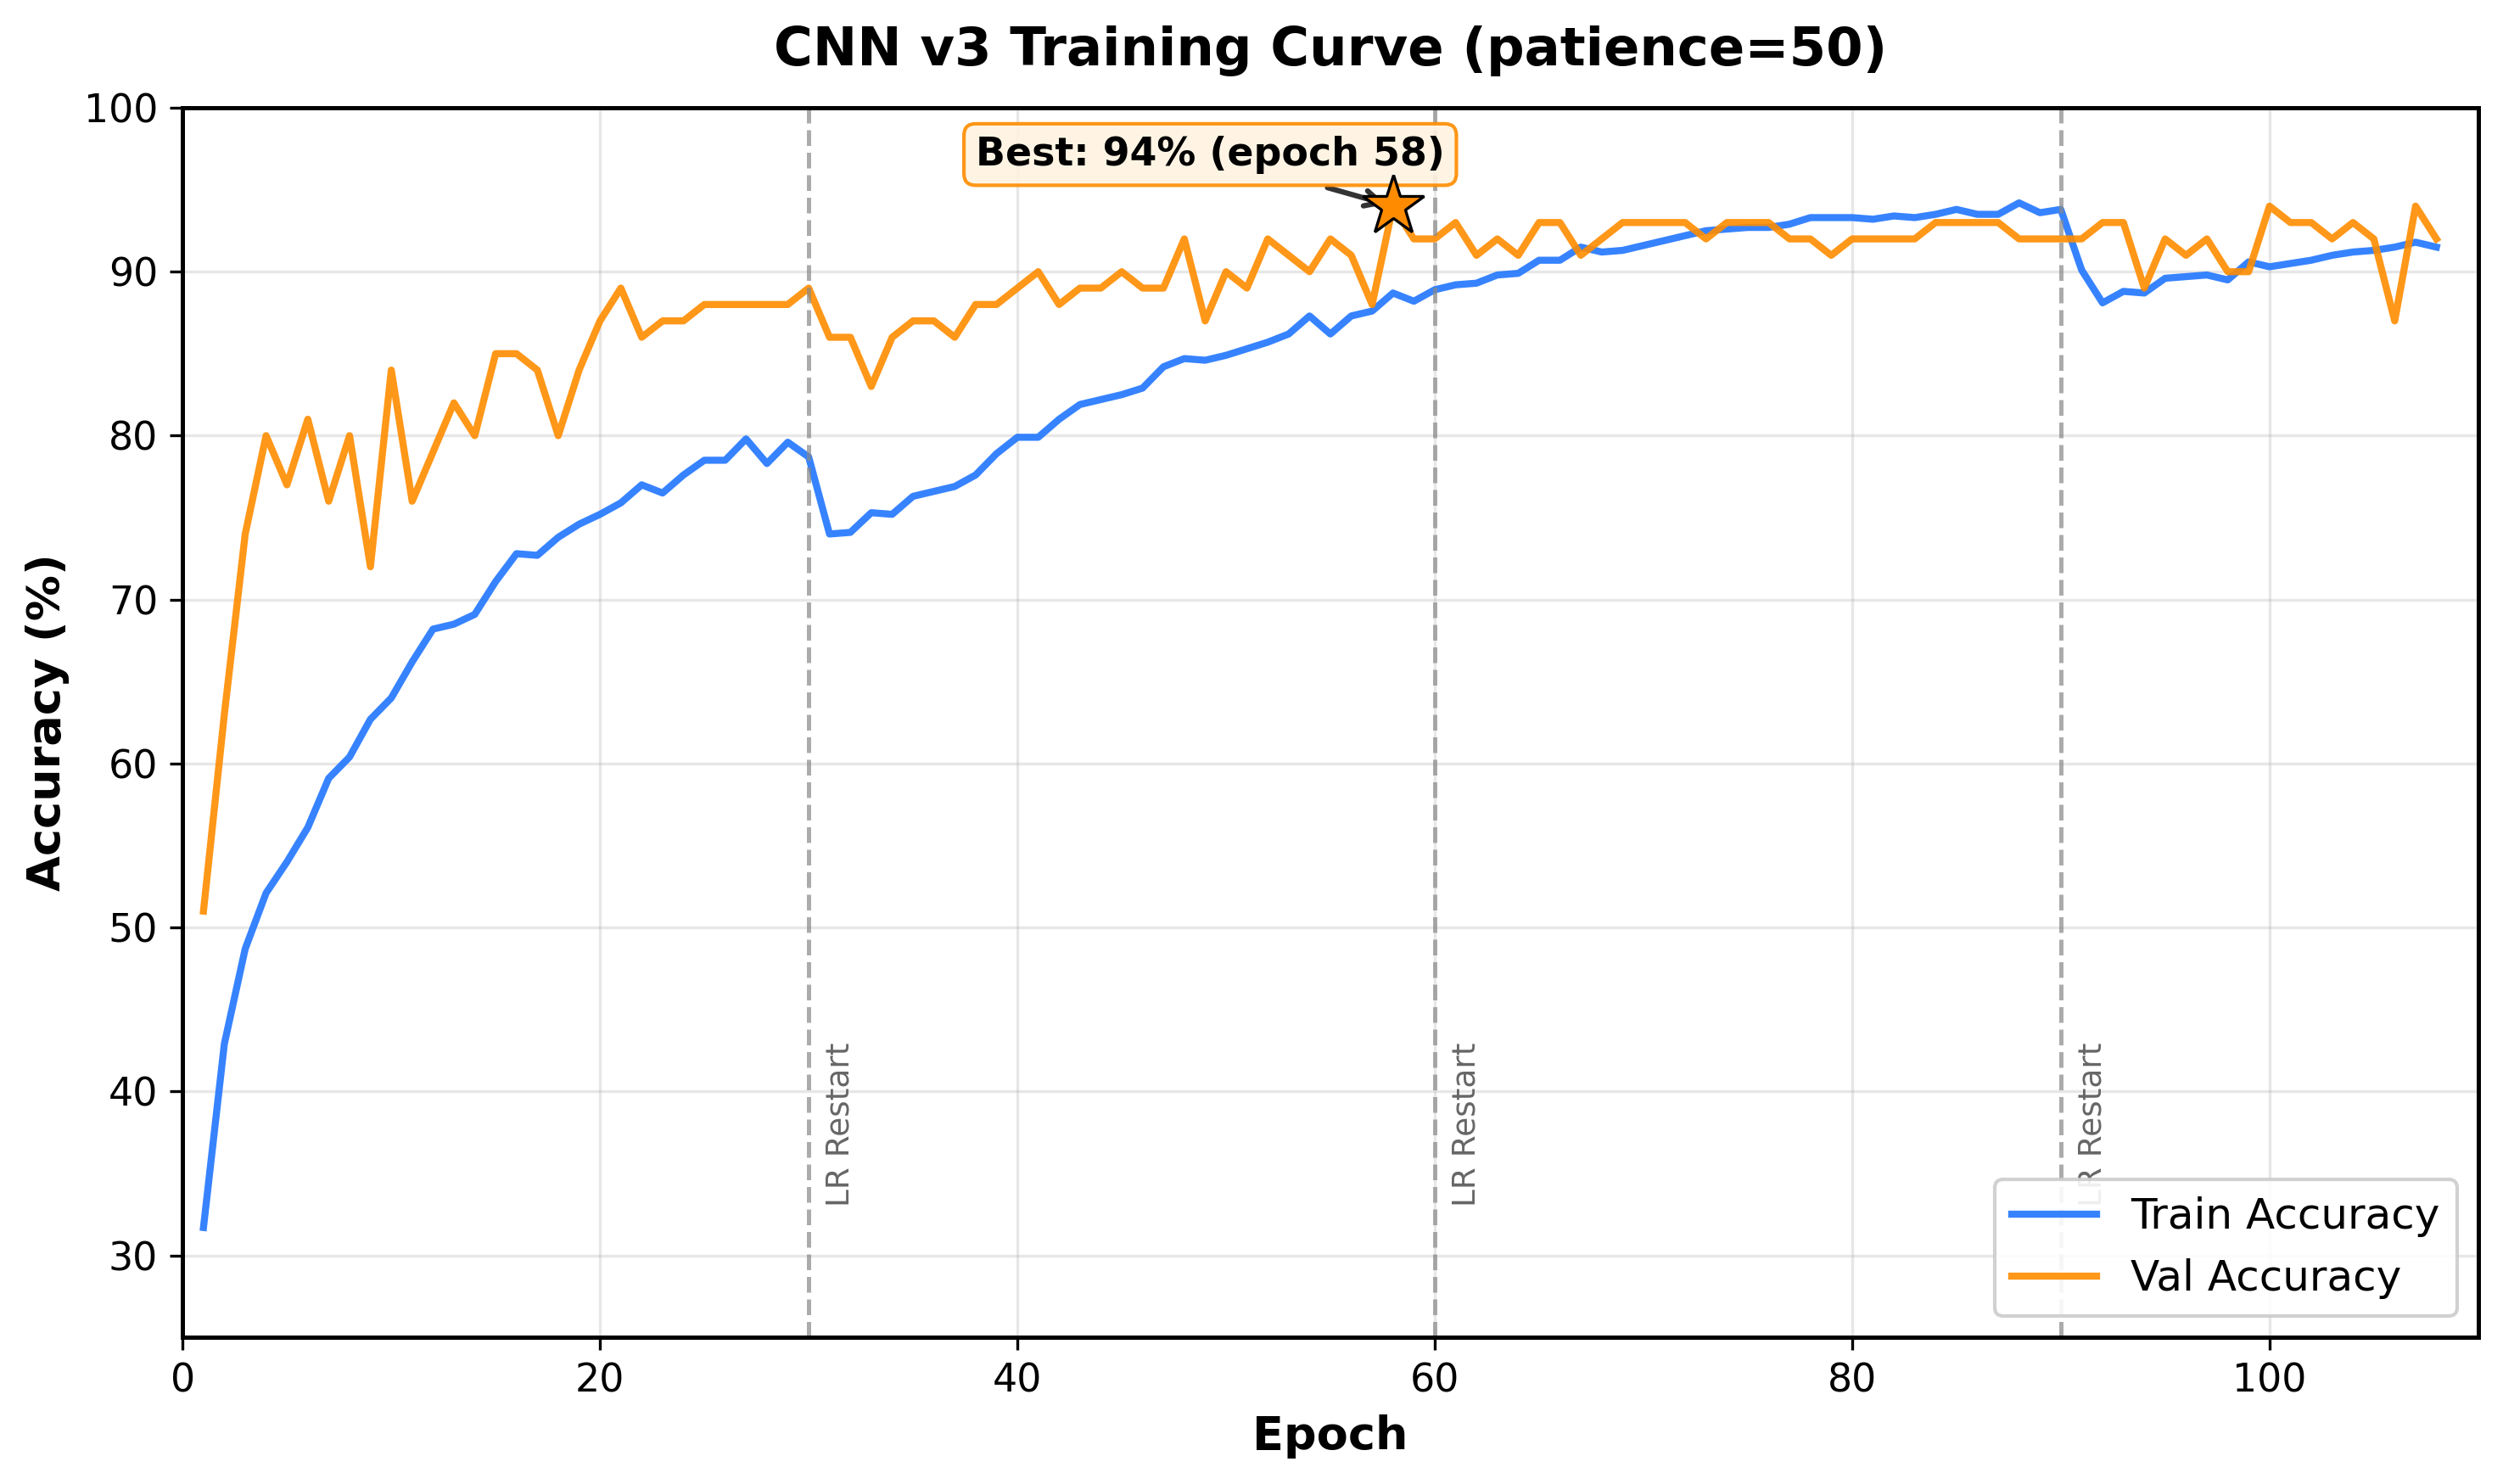
\includegraphics[width=\linewidth]{figures/training_curve.png}
\caption{Training and validation accuracy curves for CNN v3 (v3\_long variant, patience=50). Vertical dashed lines mark CosineAnnealingWarmRestarts LR resets at epochs 30, 60, and 90. The star indicates the best validation accuracy (94\% at epoch 58). The original v3 (patience=30) shows the same trajectory but peaks at epoch 67.}
\label{fig:training_curve}
\end{figure}

\textbf{A note on evaluation methods.} During training, validation accuracy is computed by majority voting over segment-level argmax predictions, yielding 94\%. At inference time, we instead average segment-level softmax probabilities before taking the argmax, which gives 92\% for a single model. The 2-point gap arises because majority voting is more robust to individual outlier segments, while probability averaging can be swayed by high-confidence wrong predictions. Our ensemble (Section~\ref{sec:ensemble}) closes this gap back to 94\%, confirming that the architecture genuinely achieves this level of performance.

\subsection{Experiment 4: Trying to Break Through 94\%}

With the architecture fixed, we tried two more things:

\begin{table}[h]
\centering
\caption{Attempts to push beyond 94\%. All use the CNN v3 architecture.}
\label{tab:ablation}
\begin{tabular}{@{}lccc@{}}
\toprule
Variant & Change & Val Acc & Best Epoch \\
\midrule
v3 (baseline) & patience=30 & 94\% & 67 \\
v3\_long & patience=50 & 94\% & 58 \\
v3\_augment & + SpecAugment~\cite{park2019specaugment} & 94\% & 48 \\
\bottomrule
\end{tabular}
\end{table}

\textbf{Longer training} (v3\_long): we increased early stopping patience from 30 to 50 epochs, hypothesizing that the original v3 had stopped too early---its early stop triggered at epoch 97, mid-way through the second cosine cycle. With more patience, the model found its best at epoch 58 but still plateaued at 94\%. The extra epochs explored the same loss landscape without discovering a better minimum.

\textbf{SpecAugment~\cite{park2019specaugment}} (v3\_augment): mild frequency/time masking ($F$=$T$=10, 50\% probability). Same 94\% ceiling, but convergence was 10 epochs faster (best at epoch 48 vs.\ 58). This acceleration makes sense: by randomly masking parts of the spectrogram, SpecAugment forces the model to learn redundant representations earlier, reducing its reliance on any single time-frequency region. However, random temporal cropping already provides substantial augmentation (10 different 3-second views per song per epoch), so the additional regularization from SpecAugment has diminishing returns.

Neither attempt broke through 94\%. The bottleneck is likely not regularization or training duration, but the representational limit of a 4-layer CNN on 3-second segments---the model cannot capture long-range temporal structure (e.g., verse-chorus transitions) that might help disambiguate the remaining 6 confusing samples.

\subsection{Experiment 5: Soft Voting Ensemble}
\label{sec:ensemble}

We ensembled v3\_long and v3\_augment via soft voting (averaging softmax probabilities). Val accuracy: 94\%---no improvement.

Looking at the individual errors: the two models misclassified the \emph{exact same 6 samples}. This makes sense---they share the same architecture, same training data, and differ only in mild augmentation. Their decision boundaries are nearly identical, so averaging their outputs changes almost nothing.

For ensemble to help, we would need genuinely diverse models: different architectures (e.g., CNN + Transformer), different input features (mel + MFCC), or different training splits. Simply toggling SpecAugment~\cite{park2019specaugment} does not create enough diversity.

\subsection{Error Analysis}

The 6 misclassified val samples are listed in Table~\ref{tab:errors}.

\begin{table}[h]
\centering
\caption{The 6 validation errors. All reflect known genre overlaps.}
\label{tab:errors}
\begin{tabular}{@{}llll@{}}
\toprule
Sample & True & Predicted & Why \\
\midrule
00930.au & rock & disco & Strong beat + electric guitar \\
00931.au & country & reggae & Similar relaxed rhythm \& texture \\
00698.au & hiphop & disco & Shared percussive patterns \\
00112.au & hiphop & rock & Electric guitar sample in the track \\
00048.au & reggae & rock & Guitar-heavy reggae \\
00597.au & pop & hiphop & Pop with hip-hop production style \\
\bottomrule
\end{tabular}
\end{table}

These are not random mistakes. As Aucouturier and Pachet~\cite{aucouturier2003representing} extensively discussed, musical genres are inherently fuzzy and subjective, with significant acoustic overlap between categories. The rock$\leftrightarrow$disco confusion reflects shared instrumentation (electric guitar + strong drums). The pop$\to$hiphop error mirrors a real-world trend where modern pop borrows heavily from hip-hop production. Sturm~\cite{sturm2013gtzan} has documented that such boundary ambiguities are particularly prevalent within the GTZAN dataset.

\begin{figure}[h]
\centering
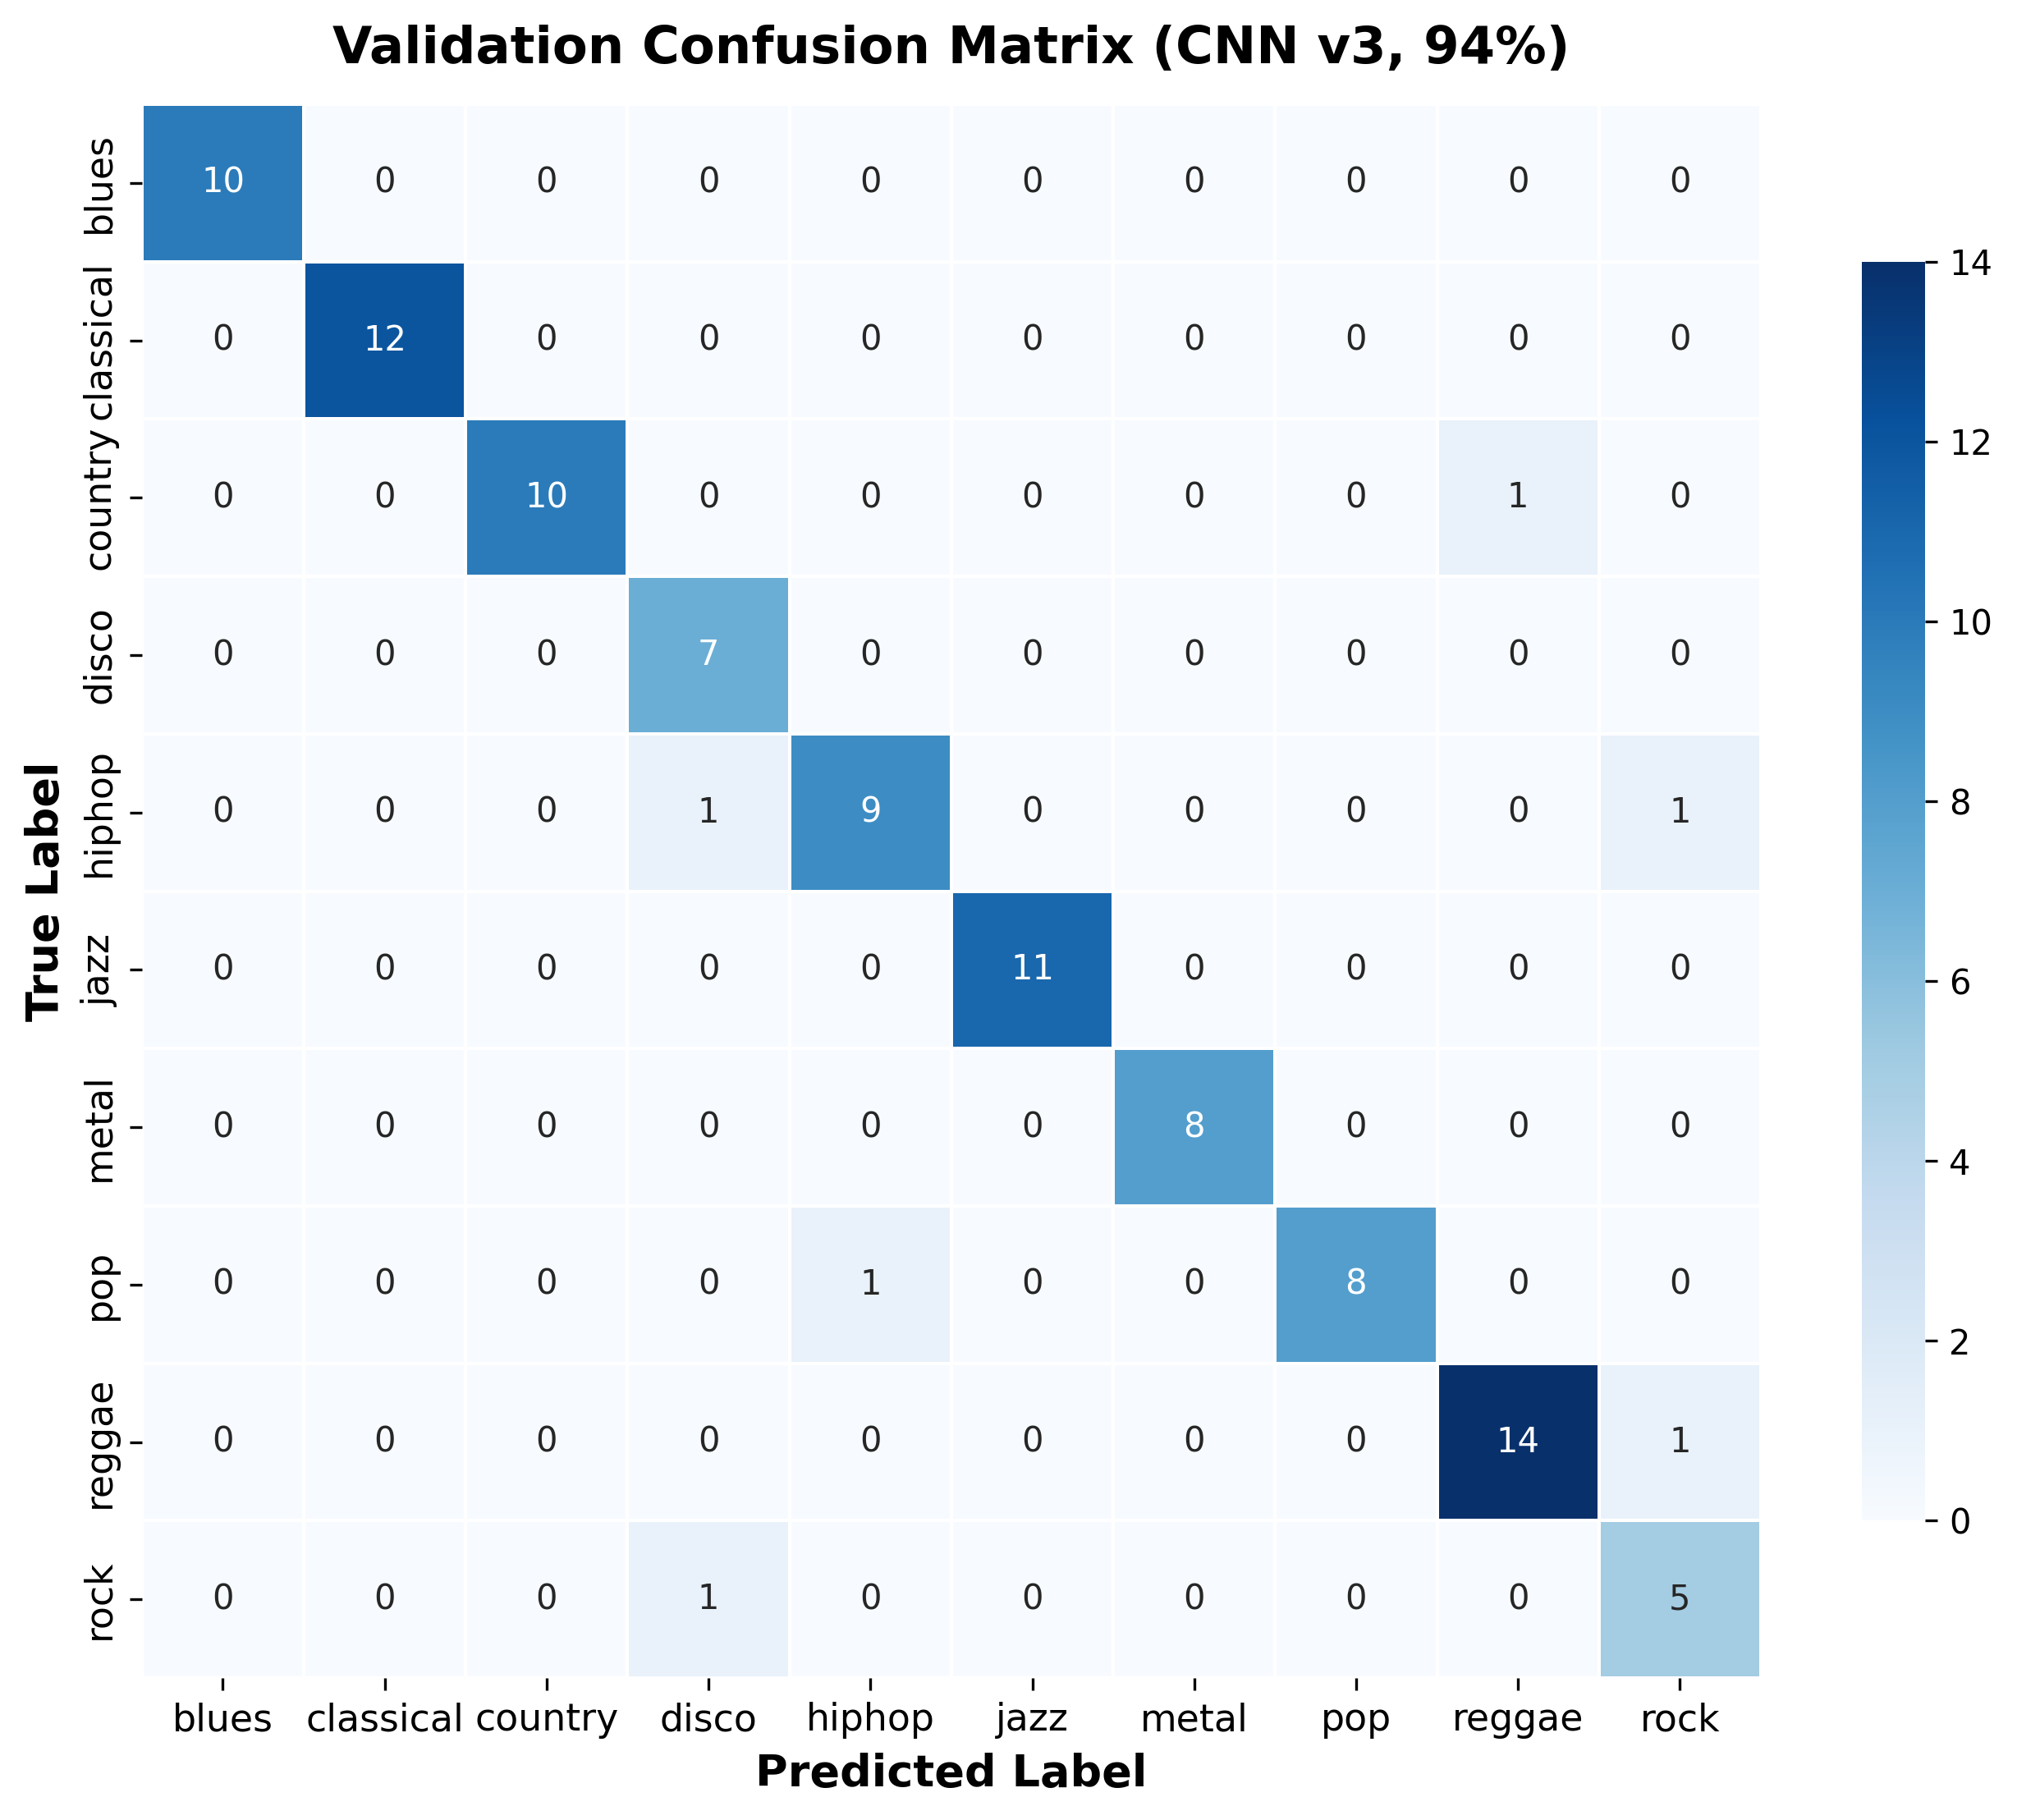
\includegraphics[width=\linewidth]{figures/confusion_matrix.png}
\caption{Confusion matrix on the validation set (CNN v3, 94\% accuracy). Off-diagonal entries correspond to the 6 errors in Table~\ref{tab:errors}.}
\label{fig:confusion_matrix}
\end{figure}

The confusion matrix (Figure~\ref{fig:confusion_matrix}) and per-class accuracy (Table~\ref{tab:perclass}) confirm this pattern: genres with distinctive sonic signatures---classical, metal, jazz---are classified perfectly, while genres that share production styles---hip-hop, rock, pop---suffer.

\begin{table}[h]
\centering
\caption{Per-class validation accuracy.}
\label{tab:perclass}
\begin{tabular}{@{}lcc@{}}
\toprule
Genre & Correct / Total & Accuracy \\
\midrule
Blues & 10 / 10 & 100\% \\
Classical & 12 / 12 & 100\% \\
Country & 10 / 11 & 90.9\% \\
Disco & 7 / 7 & 100\% \\
Hip-hop & 9 / 11 & 81.8\% \\
Jazz & 11 / 11 & 100\% \\
Metal & 8 / 8 & 100\% \\
Pop & 8 / 9 & 88.9\% \\
Reggae & 14 / 15 & 93.3\% \\
Rock & 5 / 6 & 83.3\% \\
\midrule
\textbf{Overall} & \textbf{94 / 100} & \textbf{94\%} \\
\bottomrule
\end{tabular}
\end{table}

% ============================================================
% 5. CONCLUSION
% ============================================================
\section{Conclusion}

We developed a CNN-based genre classifier that reaches 94\% on GTZAN, up from the 70\% LSTM baseline. The path was not linear---three of our experiments made things worse before we figured out why. The main lessons:

\begin{enumerate}
  \item \textbf{Don't trust the first good number.} Our 91\% model had memorized intros. Temporal ensemble---which should help---actually exposed this by dropping accuracy. Always check whether your evaluation setup matches how the model will be used.

  \item \textbf{Capacity must match data complexity.} Random cropping is the right training strategy, but it multiplies intra-class variance. A small model (102K params) that worked fine on fixed crops completely failed under random crops. The 22-point jump from 72\% to 94\% came from model capacity, not clever tricks.

  \item \textbf{Ensemble needs diversity.} Two models with the same architecture and the same training data produce the same errors. We confirmed this empirically: both models missed the exact same 6 samples. Ensemble is not a free lunch.

  \item \textbf{Some errors are not errors.} The remaining 6\% misclassification rate reflects genuine genre ambiguity~\cite{sturm2013gtzan}---hip-hop tracks with rock guitar samples, pop songs with hip-hop beats. These are songs that even humans might disagree on, as genre boundaries are inherently fuzzy and subjective~\cite{aucouturier2003representing}.
\end{enumerate}

To push further, one would likely need pretrained audio representations (e.g., HuBERT~\cite{hsu2021hubert}, CLAP~\cite{wu2023clap}) or architecturally different models for genuine ensemble diversity.

% ============================================================
% REFERENCES
% ============================================================

{\small
\begin{thebibliography}{10}

\bibitem{tzanetakis2002musical}
G.~Tzanetakis and P.~Cook,
``Musical genre classification of audio signals,''
\emph{IEEE Trans.\ Speech Audio Process.}, vol.~10, no.~5, pp.~293--302, 2002.

\bibitem{sturm2013gtzan}
B.~L.~Sturm,
``The GTZAN dataset: Its contents, its faults, their effects on evaluation, and its future use,''
\emph{arXiv:1306.1461}, 2013.

\bibitem{choi2016automatic}
K.~Choi, G.~Fazekas, M.~Sandler, and K.~Cho,
``Automatic tagging using deep convolutional neural networks,''
in \emph{Proc.\ ISMIR}, 2016.

\bibitem{dieleman2014end}
S.~Dieleman and B.~Schrauwen,
``End-to-end learning for music audio,''
in \emph{Proc.\ ICASSP}, pp.~6964--6968, 2014.

\bibitem{woo2018cbam}
S.~Woo, J.~Park, J.-Y.~Lee, and I.~S.~Kweon,
``CBAM: Convolutional block attention module,''
in \emph{Proc.\ ECCV}, pp.~3--19, 2018.

\bibitem{park2019specaugment}
D.~S.~Park \emph{et al.},
``SpecAugment: A simple data augmentation method for automatic speech recognition,''
in \emph{Proc.\ Interspeech}, pp.~2613--2617, 2019.

\bibitem{loshchilov2017sgdr}
I.~Loshchilov and F.~Hutter,
``SGDR: Stochastic gradient descent with warm restarts,''
in \emph{Proc.\ ICLR}, 2017.

\bibitem{mcfee2015librosa}
B.~McFee \emph{et al.},
``librosa: Audio and music signal analysis in Python,''
in \emph{Proc.\ SciPy}, pp.~18--24, 2015.

\bibitem{hsu2021hubert}
W.-N.~Hsu \emph{et al.},
``HuBERT: Self-supervised speech representation learning by masked prediction of hidden units,''
\emph{IEEE/ACM Trans.\ Audio, Speech, Lang.\ Process.}, vol.~29, pp.~3451--3460, 2021.

\bibitem{wu2023clap}
Y.~Wu \emph{et al.},
``Large-scale contrastive language-audio pretraining with feature fusion and keyword-to-caption augmentation,''
in \emph{Proc.\ ICASSP}, 2023.

\bibitem{chen2016xgboost}
T.~Chen and C.~Guestrin,
``XGBoost: A scalable tree boosting system,''
in \emph{Proc.\ ACM SIGKDD}, pp.~785--794, 2016.

\bibitem{silla2007ensemble}
C.~N.~Silla~Jr., A.~L.~Koerich, and C.~A.~A.~Kaestner,
``Automatic music genre classification using ensemble of classifiers,''
in \emph{Proc.\ IEEE International Conference on Systems, Man and Cybernetics}, pp.~1687--1692, 2007.

\bibitem{aucouturier2003representing}
J.-J.~Aucouturier and F.~Pachet,
``Representing musical genre: A state of the art,''
\emph{Journal of New Music Research}, vol.~32, no.~1, pp.~83--93, 2003.

\end{thebibliography}
}

% ============================================================
% END OF REPORT
% ============================================================
